\section{Introduction}
\label{sec:intro}

% The emergence of a new breed of computer
Embedded devices are growing impressively in popularity and ubiquity in recent years.
This growth can be attributed to the emergence of new application domains inspired by small,
highly resource-limited programmable processors known as microcontroller units (or MCUs),
which may have as little as a few kilobytes of RAM. It is now the case that less than 1 percent of
the world's processors reside in general purpose computers such as desktop PCs, laptops and tablets
- with MCUs picking up the remainder~\cite{borriello2000embedded}.
Furthermore, demand for MCUs continues to grow due to their use in the monitoring and
control of a wide variety of systems, ranging from wearables, to home automation,
industrial automation, and smart grids - a phenomenon broadly referred to as the Internet of Things (IoT).

MCUs are highly resource limited devices, but are not simply smaller versions of laptop and desktop machines.
They are architecturally quite distinct. If we are to undertand how to optimize
programming languages and their implementation for such devices it is worth dwelling on the key characteristics of MCUs, namely their storage and CPU capabilities. 
Table \ref{table:devices} highlights the core capabilities of MCU-based devices
vs. a typical PC.

\begin{table}[]
    \centering
    \begin{tabular}{|l|r|r|r|r|r|r|}
    \hline
                           &          &              & \bf{Word}  & \bf{CPU} &            \\
    \bf{Device}            & \bf{RAM} & \bf{Flash}   & \bf{Size}  & \bf{Speed} & \bf{CPU}  \\ \hline
    Uno            & 2 KB       & 32 KB      & 8          & 16MHz & AVR       \\ \hline
    micro:bit          & 16 KB      & 256 KB     & 32         & 16MHz & Cortex     \\ \hline
    CPX           & 32 KB      & 256 KB     & 32         & 48MHz & Cortex    \\ \hline
    PC             & 16 GB      & 1 TB       & 64         & 3GHz & Intel      \\ \hline
    \end{tabular}
    \caption{\label{table:devices}Example microcontroller devices in relationship to a typical PC. Device abbreviations: Uno (Arduino Uno), micro:bit (BBC micro:bit), CPX (Adafruit Circuit Playground Express); PC (Personal Computer).}
    \end{table}

While it is clear that all such devices are highly resource contrained compared to modern PCs
(about six orders of magnitude less on most metrics), a deeper analysis derives two further observations.

Firstly, \emph{MCUs are processor rich}. Contrary to first impressions, these devices have
a \emph{proportionally} large amount of processing power. Consider the BBC micro:bit
versus a typical PC. It has about 100 times less CPU power, but 10\textsuperscript{6} times less RAM,
and 10\textsuperscript{6} time less storage. A language/runtime designed for MCUs should therefore not
only seek to provide high code density and spatial efficiency,
\emph{but to actively trade off time for space}, where possible.

Secondly, \emph{MCUs are accumulating more features on chip}.
MCUs still follow Moore's law (the number of transistors doubles roughly every two years).
However, this additional capacity is
not typically invested in simply optimizing processing power. Instead, \emph{independent peripherals}
are integrated onto the same MCU as the CPU. Examples include integrated radio hardware such
as Bluetooth/WiFi and audio inputs and outputs. This hardware is designed to run independently of the
CPU, hence an effective language/runtime should directly support \emph{an asynchronous
interaction model}.

% Despite this languages and programming environments have yet to keep pace with the mainstream (e.g. Arduino/mbed)
Furthermore, with this surge in the demand for MCUs across a wide spectrum of applications,
there is a need to simplify the programming of such devices so that more people can participate in
the creation of MCU-based systems. From rapid product innovation to making and education,
we have seen a sustained growth in the volume and diversity of people wishing to program MCU-based devices. These new application developers share a common characterisitic - \emph{they are typically not professional software developers}~\cite{dougherty2012maker,bruce2015make,maksimovic2014raspberry}.

Programming languages and development environments for MCUs have not kept pace with advances
in hardware and diversification of user domains. Elsewhere, we have long supported inexperienced developers through languages such as Java, C\#, Python and JavaScript, and also
through visual programming frameworks such as Blockly~\cite{Blocky2015}.

In the world of the MCU, the C/C++ languages remain the standard, and for good reasons:
they provide a familiar imperative programming model, with compilers that produce highly efficient code, and enable low level access to hardware features when necessary. Popular examples
include the Arduino project (\url{www.arduino.cc})~\cite{buildingArduino2014},
started in 2003, and ARM's Mbed platform (\url{www.mbed.org})~\cite{ARMmbed} - both of which rely heavily on a C/C++ programming model. However, the limitations of using C/C++ as an application programming language for
\emph{inexperienced} developers are well understood~\cite{blikstein2013gears}.

% Paper overview
We introduce a novel architecture for MCU-based devices,
that is designed with three aspirational goals in mind:
(1) it should be usable by \emph{anyone}, not just trained professionals;
(2) it should be available \emph{anywhere}, requiring no specialized software (native applications
or device drivers) to operate;
(3) it should run efficiently on \emph{anything}, from devices with as little as 2KB of memory.

This paper focuses on the design, implementation, and evaluation of this architecture using the devices listed in Table~\ref{table:devices} as exemplars. We leave a detailed treatment about usability for future work.
More specifically, we present and evaluate a platform that bridges the worlds of the web and the
MCU through three novel technologies:

\begin{itemize}
\item \emph{\MCN}, a web application containing an \emph{in-browser compiler} that supports the
simplified programming of MCUs via editors for visual blocks and textual JavaScript languages
(Section~\ref{sec:makecode});

\item \emph{Static TypeScript}, a statically-typed subset of TypeScript
(\url{www.typescriptlang.org}) that we have defined for fast execution on low-memory devices,
with a simple model for linking against pre-compiled C++ (Section~\ref{sec:sts});

\item \emph{\CO}, a component-based, event-driven, fiber-based C++ runtime environment
that bridges the semantic gap between higher-level languages (such as TypeScript) and the hardware,
modelling each hardware component as a software component (Section~\ref{sec:codal});
\end{itemize}
Our results (Section~\ref{sec:evaluate}) show that these technologies combined can enable simplified programming through modern
languages and event-based constructs while maintaining a relatively high degree of temporal and spatial efficiency.
We demonstrate up to 50x better performance than other state-of-the-art implementations,
in some cases nearing the performance of native C++.  The platform was deployed about a year
ago and sees daily use by thousands of users.

\subsection{Architectural Overview}

\begin{figure}[t]
    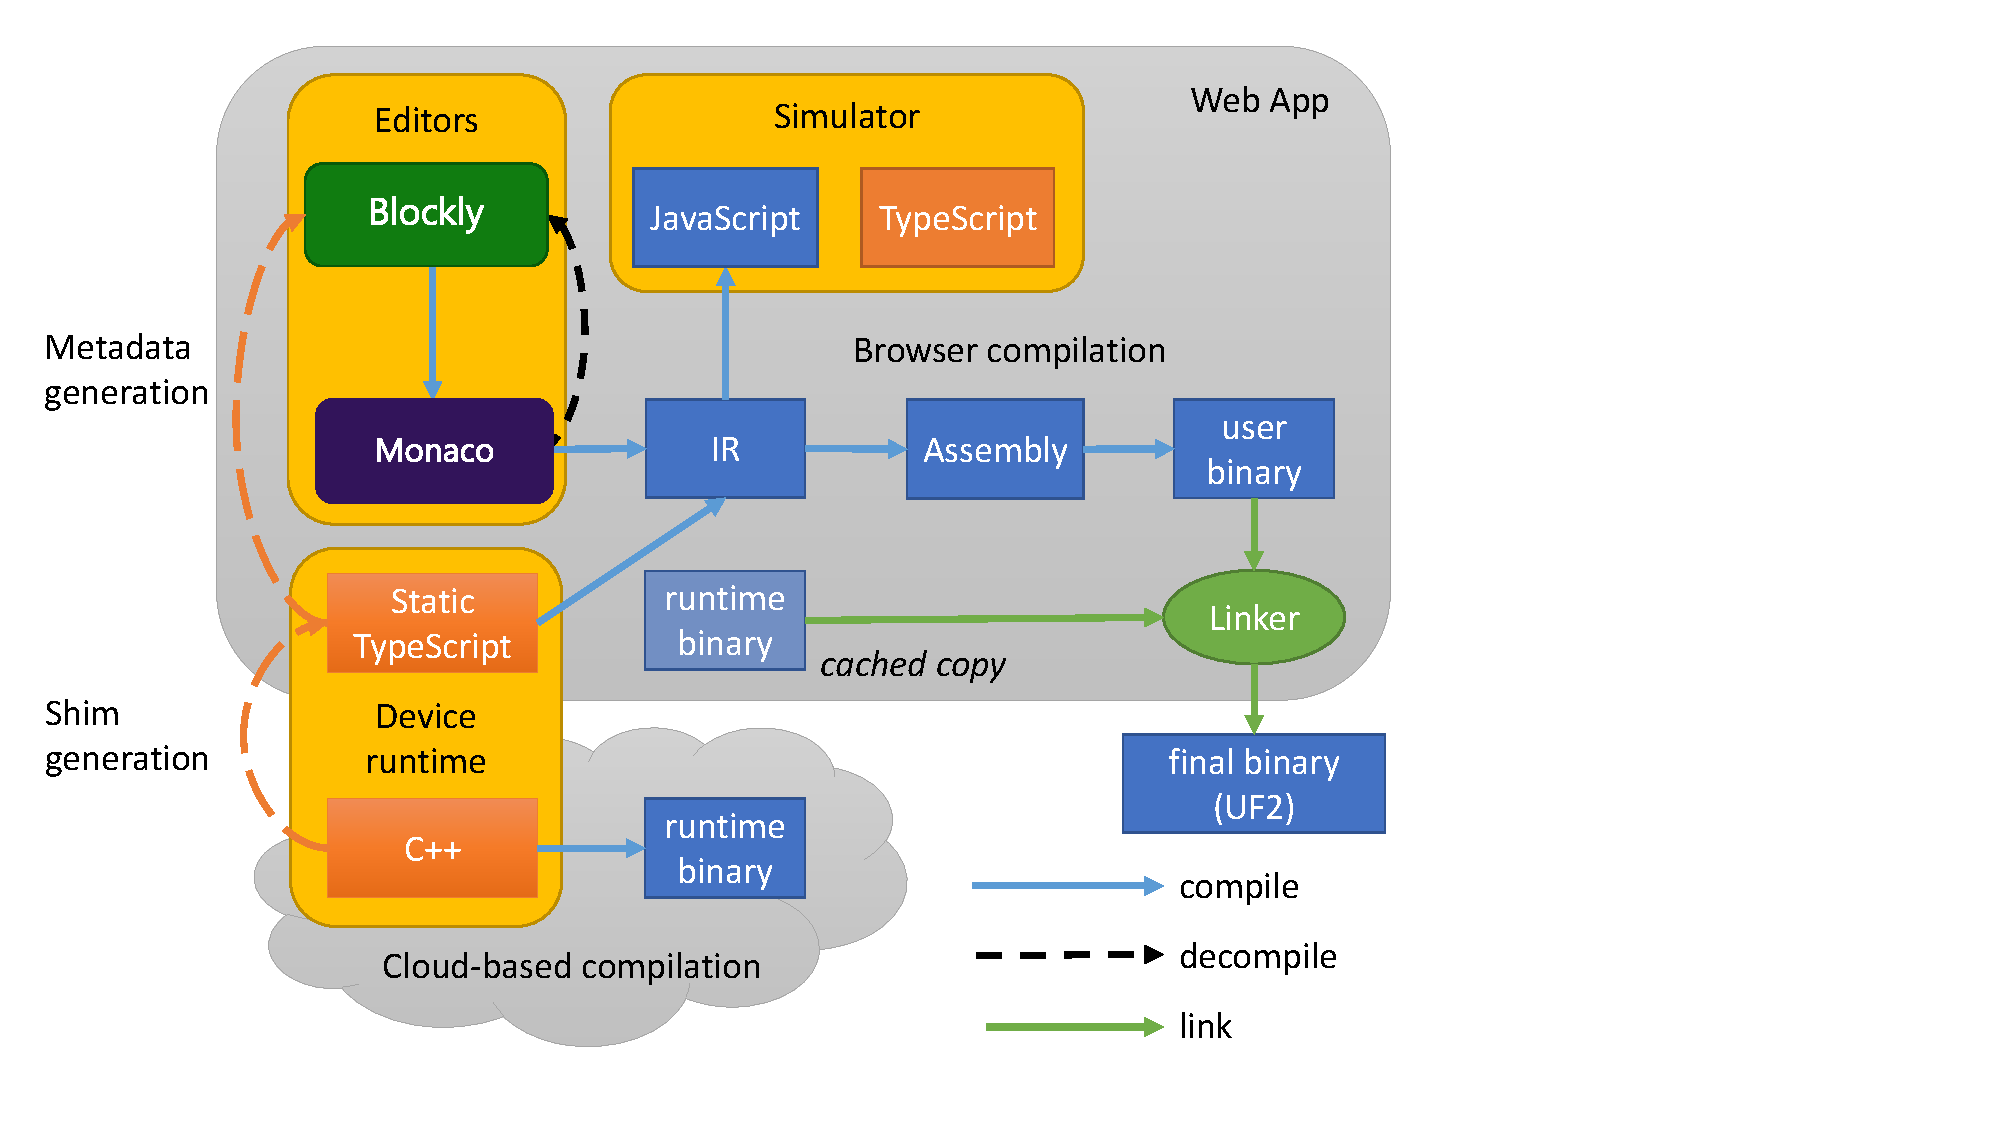
\includegraphics[width=4.8in]{makecodeFig.pdf}
\caption{\label{fig:makecode}\MC web app}
\end{figure}

Currently, due to the low-level nature of MCU programming, additional drivers and software are commonly required to be locally installed in order to program them. In restricted environments, like libraries and schools, safeguards are put in place to protect users and machines from downloading or installing additional software. Further, Internet connections are unrealiable in remote locations. These factors create barriers for designing a programming environment that runs \emph{anywhere}. Therefore, a solution is required that can: (1) operate in restricted environments; (2) operate with little, or no internet connectivity; and (3) work on any operating system.

To meet these requirements, we created the \MC web app (Figure~\ref{fig:makecode}), the entry point of the platform. The web app can be accessed from any modern web browser and cached locally for \emph{entirely offline use}. The \MC web app incorporates the open source Blockly (\emph{\href{https://github.com/google/blockly}{blockly}}) and Monaco (\emph{\href{https://github.com/Microsoft/monaco-editor}{monaco-editor}}) editors (upper-left), an in-browser device simulator (upper-right) for testing programs before transfering them to the physical device, as well as \emph{in-browser compilation} of Static TypeScript to machine code and linking against the C++ runtime (\emph{\CON}), pre-compiled (by a cloud service, lower left). The statically-typed runtime and type inference on user code allows users to write code that looks like plain JavaScript (see Figure~\ref{fig:example}).

\MC devices appear as USB pen drives when plugged into a computer. After a user has finished developing a program, the compiled binary is ``downloaded'' locally to the users computer and then transferred (flashed) to the MCU (exposed as USB pen drive) by a simple file copy operation. No additional installation is required to program the MCU as drivers for pen drive come pre-installed on many operating systems (MacOS, Windows, Linux, Android, ChromeOS).

These advances enable beginners to get started programming MCUs from any modern web browser, and offer a safe environment for hardware vendors to innovate and add new components using Static TypeScript. All of the platform's components are open source on GitHub.

\subsection{Running Example: firefly simulation.}

Figure~\ref{fig:example} shows a JavaScript
program that implements a simple ``firefly'' example
for the Adafruit Circuit Playground Express (CPX), which has an onboard light sensor and 10 RGB LEDs (among other sensors and output devices).

This program demonstrates an emergent, time-based algorithm, run on multiple CPXs in a dark environment. Over time they will synchronize to a common clock using light pulses --- akin to fireflies synchronizing their blinking in the wild.

% INCLUDE? (\url{https://www.youtube.com/watch?v=sROKYelaWbo}).

At the top-level, the program has three statements:
the first initializes the global variable \emph{clock} (line 1); the
second registers an event handler (a lambda function) to execute
each time the CPX's light detector senses a bright light (line 3); the
third registers a lambda function to run forever on a fiber (line 18),
to keep track of time and pulse the CPX's 10 LEDs at regular intervals.

Note that although this program appears as a JavaScript program (there are no
types mentioned explicitly), this program also is a Static TypeScript program:
the static type of every variable and expression
can be inferred and the program (with inferred types) passes the more restrictive type checks
of Static TypeScript, as detailed in Section~\ref{sec:sts}.

The program also demonstrates the use of the non-preemptive concurrency
model supported by both \MC (for JavaScript) and \CO (for C++).
The forever procedure executes the lambda inside a ``while (true)''
loop that yields (via a call to \emph{loops.pause}) after each loop iteration.
This gives the light-detection event handler a chance to execute
upon user input (in a separate fiber). Although the global variable \emph{clock} is
shared by the two fibers, there is no data race due to the non-preemptive
scheduling model.

We will refer to this example throughout.

\begin{figure}
\begin{lstlisting}
  let clock = 0

  input.onLightConditionChanged(
    LightCondition.Bright, () => {
      if (clock < 8) {
          clock += 1    // catchup to neighbor
      }
  })

  loops.forever(() => {
    if (clock >= 8) {
        // notify neighbors
        light.setAll(Colors.White)
        loops.pause(200)
        light.clear()
        clock = 0         // reset the clock
    } else {
        loops.pause(100)
        clock += 1
    }
})
\end{lstlisting}
\caption{\label{fig:example}Running example: firefly simulation.}
\end{figure}
